\documentclass[a4paper, 11pt]{article}
\usepackage[polish]{babel}
\usepackage[T1]{fontenc}
\usepackage{hyperref}
\usepackage{array}
\usepackage{amssymb}
\usepackage{amsmath}
\usepackage{changepage}
\usepackage{multicol}
\usepackage[margin=1in]{geometry}
\hypersetup{
    colorlinks,
    citecolor=black,
    filecolor=black,
    linkcolor=black,
    urlcolor=black
}
\usepackage{graphicx}

\usepackage{tikz}
\usetikzlibrary{fit,arrows,matrix,positioning, calc, shapes.gates.logic.IEC, shapes.gates.logic.US}
\usetikzlibrary {arrows.meta}
\tikzstyle{branch}=[fill,shape=circle,minimum size=3pt,inner sep=0pt]


\title{%
        \vspace{-1cm}
       \large Sprawozdanie Laboratorium Fizyka dla informatyków \\
       \huge Wyznaczanie zależności przewodnictwa od temperatury dla półprzewodników i przewodników.}

\author{Stanisław Fiedler 160250}
\date{LAB 4, 10 grudnia 2024}

\begin{document}
\begin{table}
	\begin{adjustwidth}{-0.25\textwidth}{-0.25\textwidth}
		\begin{center}
			\begin{tabular}{|l|l|l|l|l|}
				\hline
				Nr Ćwiczenia 203                                             & Data wykonania 10.12.2024                 & Wydział WIiT & Semestr 3 & Grupa LAB L1 \\
				\hline
				\multicolumn{2}{|l|}{ Prowadzący: mgr inż. Taras Zhezhera  } & \multicolumn{2}{|l|}{ Stanisław Fiedler } & Ocena:                                  \\
				\hline
			\end{tabular}
		\end{center}
	\end{adjustwidth}
\end{table}

\maketitle
\tableofcontents

\section{Wstęp teoretyczny}\label{sec:wstep} % (fold)

Prawo Ohma mówi że gęstość prądu w dowolnym miejscu przewodnika jest wprost proporcjonalna do natężenia pola elektrycznego oraz zależy od przewodnictwa elektrycznego.
Wartość przewodnictwa jest określona bezpośrednio przez koncentrację i ruchliwość nośników.

\[
	j = \sigma E
\]

W przewodnikach koncentracja nośników jest bardzo duża i nie zależy od temperatury.
Zmianę przewodnictwa powoduje zmniejszanie się ruchliwości elektronów wraz ze wzrostem temperatury.


W półprzewodnikach nośnikami prądu są elektrony w paśmie przewodnictwa oraz dziury w paśmie walencyjnym.
Liczba elektronów w paśmie przewodzenia zależy od temperatury.
Zmiana ruchliwości nośników w półprzewodnikach ma znikomy wpływ na przewodnictwo, zależy ono przedewszystkim od koncentracji nośników.
Zwiększanie liczby nośników powoduje zmniejszenie oporu elektrycznego.


% section wstep (end)

\section{Wyniki pomiarów}\label{sec:wyniki_pomiarow} % (fold)
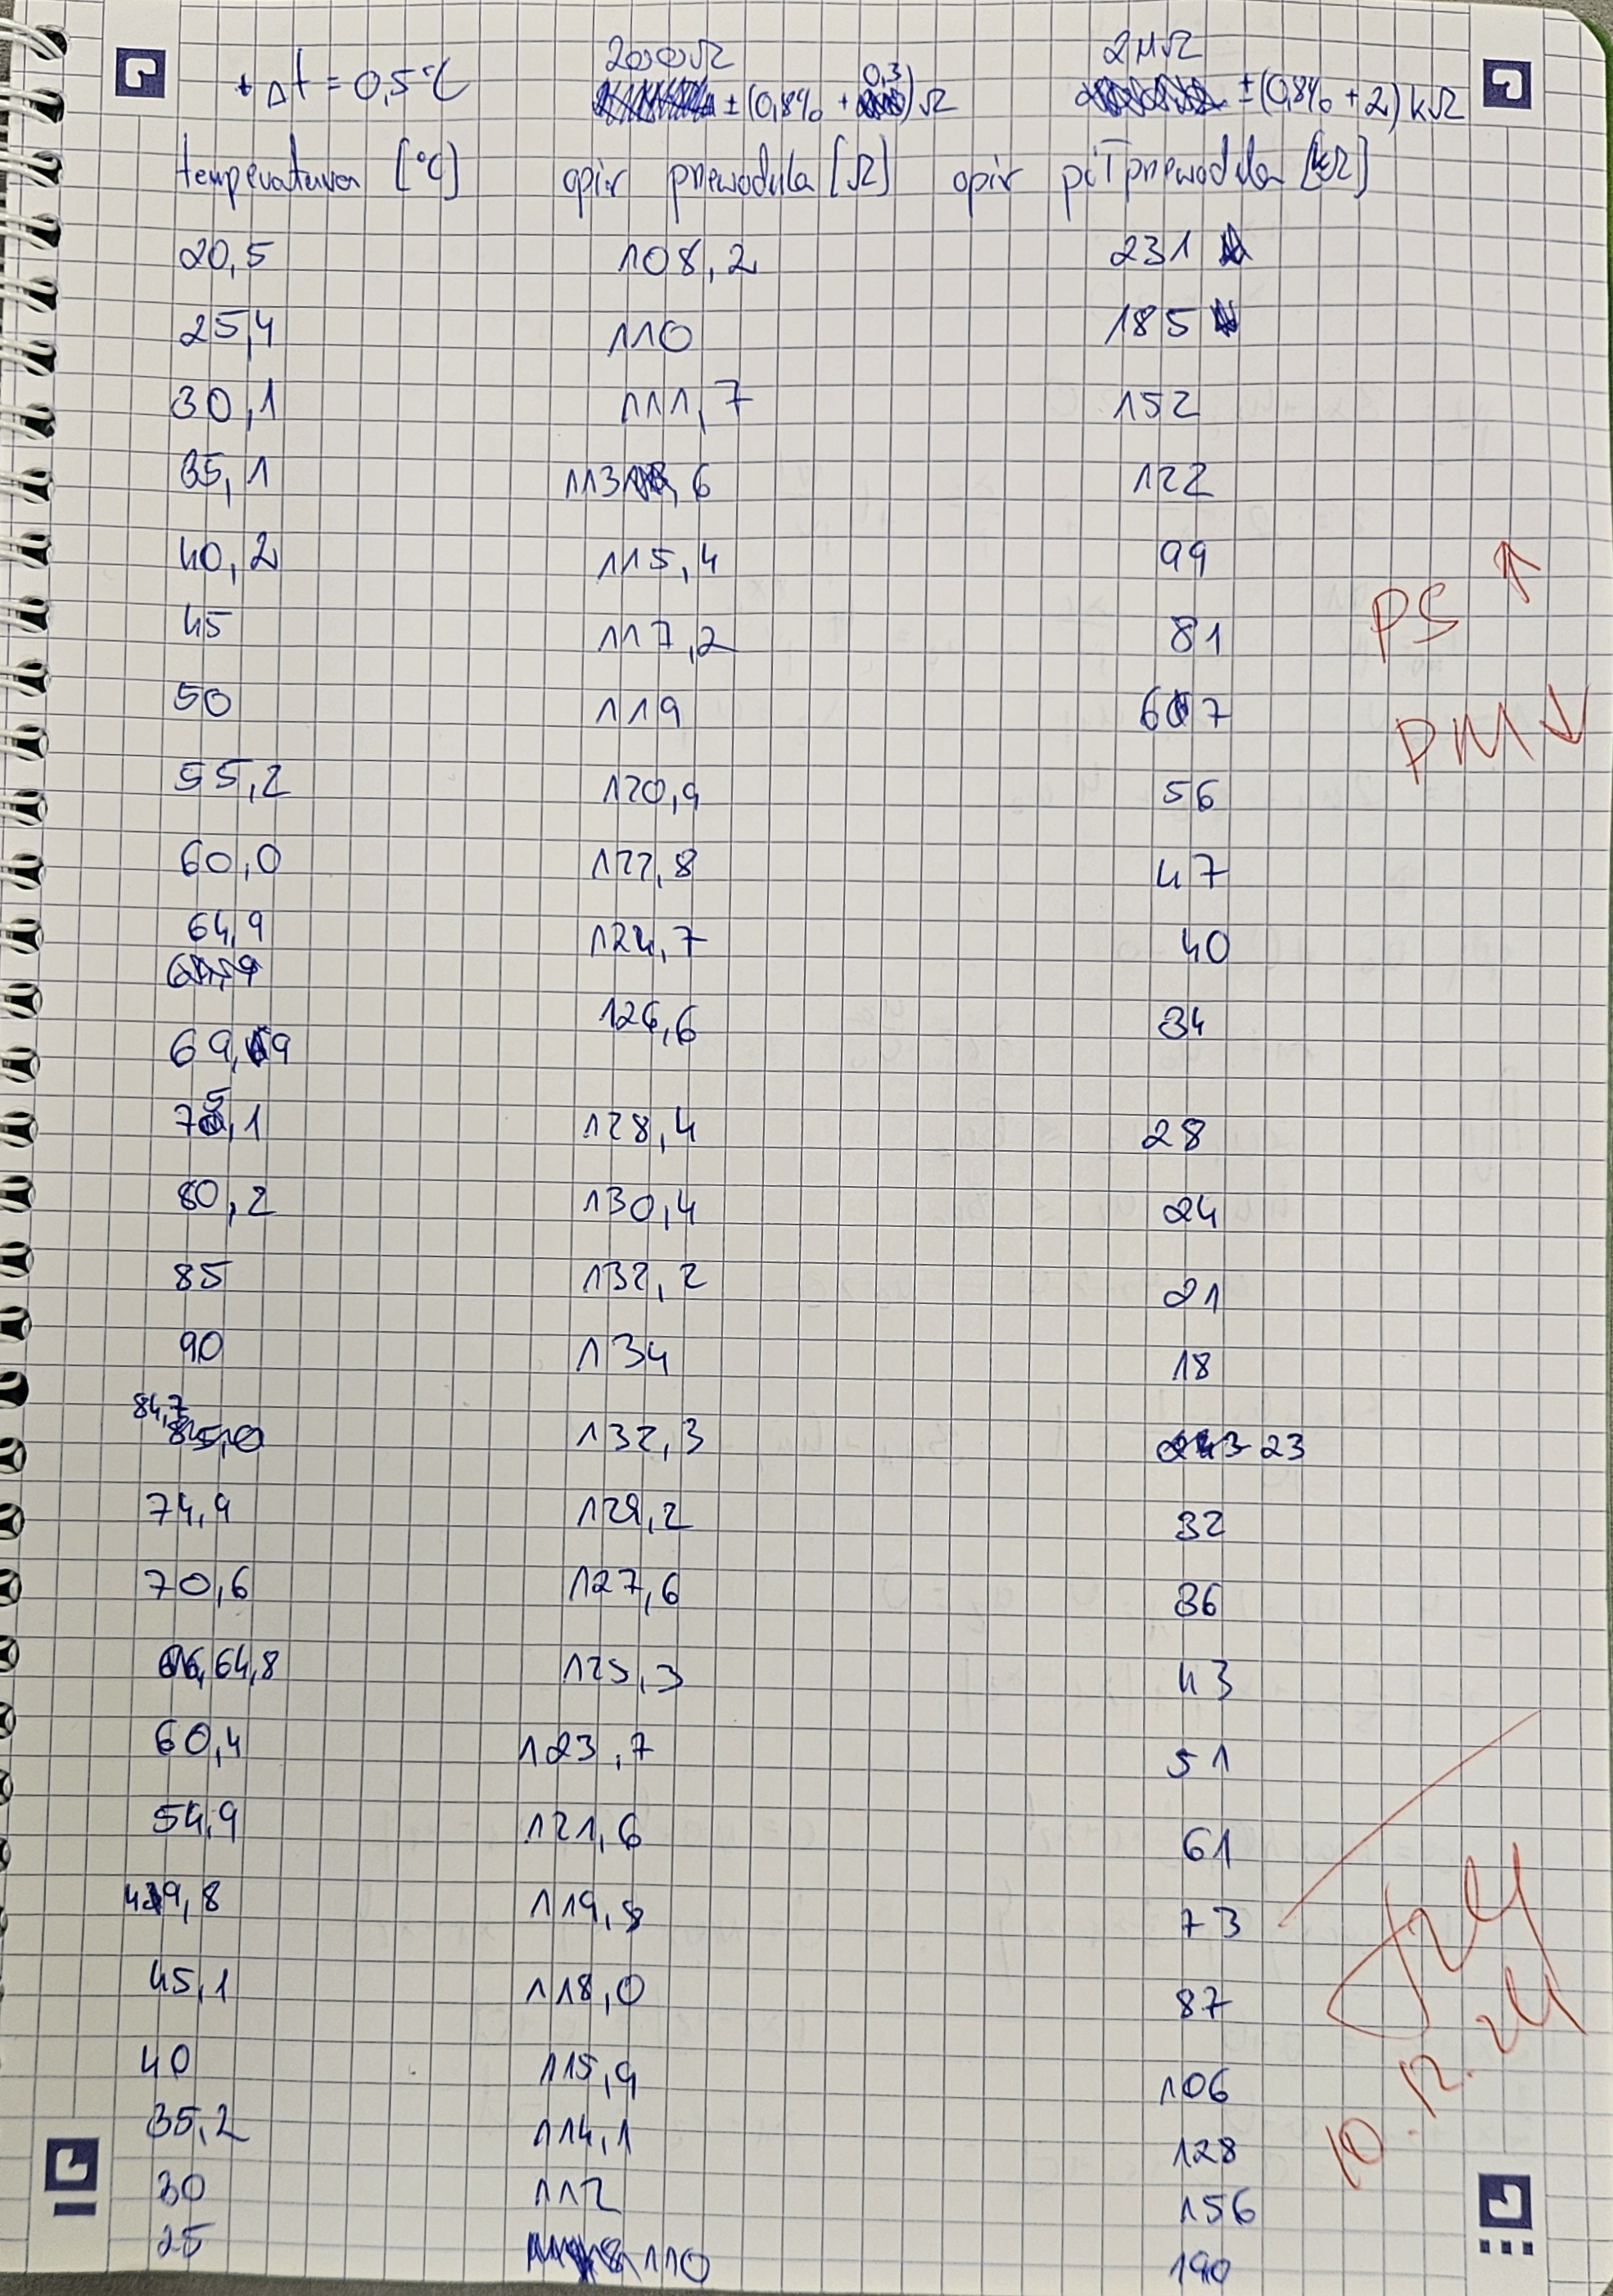
\includegraphics[scale=0.2]{images/pomiary.jpg}
\pagebreak
% subsection Zdjecie wynikow pomiarow (end)

\section{Opracowanie wyników}\label{sec:opracowanie_wynikow} % (fold)

\subsection{Wykres zaleznosci $R = f(T)$}\label{sub:wykres_zaleznosci_r_f_t_} % (fold)

\begin{minipage}{0.6\textwidth}
	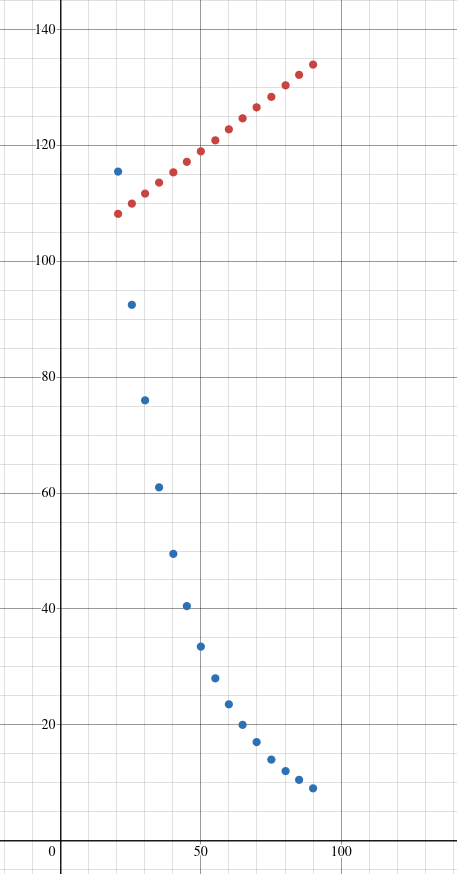
\includegraphics[scale=0.45]{images/wykres1.png}
\end{minipage}%
\begin{minipage}{0.5\textwidth}
	\begin{description}
		\item[Czerwony:] przewodnik $[\Omega]$
		\item[Niebieski:] półprzewodnik $[2k \Omega]$
	\end{description}
\end{minipage}
% subsection Wykres zaleznosci $R = f(T)$ (end)

\subsection{Energia aktywacji w półprzewodniku}\label{sub:} % (fold)
\begin{center}

	\begin{tabular}{|l|l|l|l|l|l|l|}
		\hline
		temp $[°C]$ & $K$    & opór $[k\Omega]$ & $[\Omega]$ & $R^{-1}$     & $T^{-1}$ & $ln(R^{-1})$ \\ \hline
		20.5        & 293.65 & 231              & 231000     & 4.329004E-06 & 0.003405 & -12.3501     \\ \hline
		25.4        & 298.55 & 185              & 185000     & 5.405405E-06 & 0.003349 & -12.1281     \\ \hline
		30.1        & 303.25 & 152              & 152000     & 6.578947E-06 & 0.003297 & -11.9316     \\ \hline
		35.1        & 308.25 & 122              & 122000     & 8.196721E-06 & 0.003244 & -11.7117     \\ \hline
		40.2        & 313.35 & 99               & 99000      & 1.010101E-05 & 0.003191 & -11.5028     \\ \hline
		45          & 318.15 & 81               & 81000      & 1.234567E-05 & 0.003143 & -11.3022     \\ \hline
		50          & 323.15 & 67               & 67000      & 1.492537E-05 & 0.003094 & -11.1124     \\ \hline
		55.2        & 328.35 & 56               & 56000      & 1.785714E-05 & 0.003045 & -10.9331     \\ \hline
		60          & 333.15 & 47               & 47000      & 2.127659E-05 & 0.003001 & -10.7579     \\ \hline
		64.9        & 338.05 & 40               & 40000      & 0.000025     & 0.002958 & -10.5966     \\ \hline
		69.9        & 343.05 & 34               & 34000      & 2.941176E-05 & 0.002915 & -10.4341     \\ \hline
		75.1        & 348.25 & 28               & 28000      & 3.571428E-05 & 0.002871 & -10.2399     \\ \hline
		80.2        & 353.35 & 24               & 24000      & 4.166666E-05 & 0.002830 & -10.0858     \\ \hline
		85          & 358.15 & 21               & 21000      & 4.761904E-05 & 0.002792 & -9.95227     \\ \hline
		90          & 363.15 & 18               & 18000      & 5.555555E-05 & 0.002753 & -9.79812     \\ \hline
	\end{tabular}

	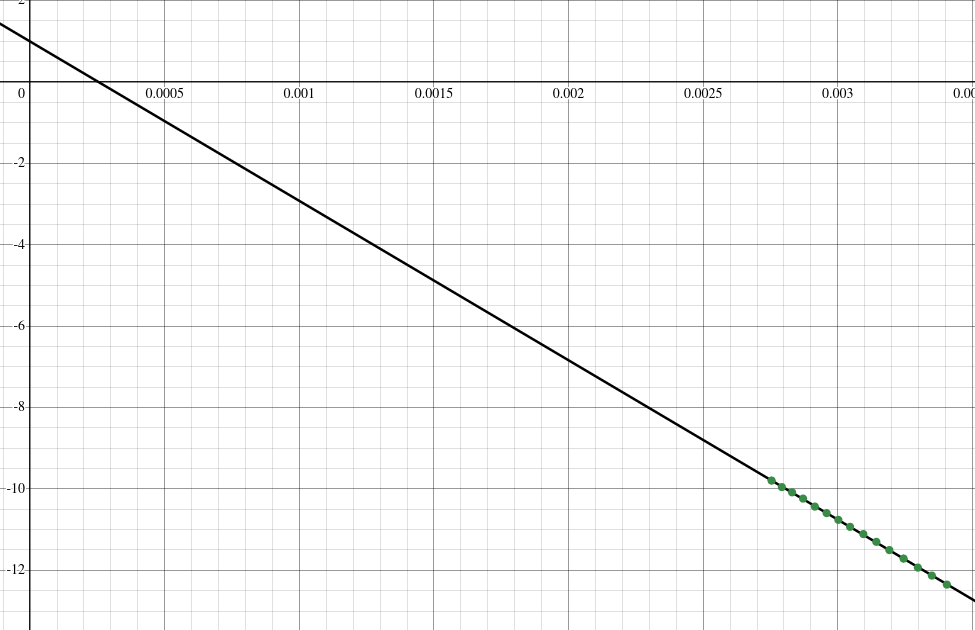
\includegraphics[scale=0.4]{images/reg_pol.png}

\end{center}
% subsection polprzewodnik (end)


Regresja liniowa została wyznaczona z użyciem Python z bibliotekami numpy oraz scipy.\
Równanie prostej ma postać:
\[
	y = -3916.94699x + 0.994993
\]
Więc współczynnik a wynosi
\[
	a = -3912.050913 \pm 13.221968
\]

Energia aktywacji wyznaczona z równia wynosi:
\[
	E_A = a \cdot k
\]
\[
	E_A = -3917 \cdot 1,38 \cdot 10^{-23} = -5,40546 \cdot 10^{-20} \quad J
\]
\[
	\Delta E_A = |a \cdot \Delta k| + |k \cdot \Delta a| \quad J
\]
\[
	\Delta E_A = | 1,38 \cdot 10^{-23} \cdot 13.221968|  = 0,0182 \cdot 10^{-20} \quad J
\]
\[
	E_A =\frac{-5,40546 \cdot 10^{-20}}{1,6 \cdot 10^{-19}} = -0.3378 \quad eV
\]
\[
	\Delta E_A = \frac{1,82 \cdot 10^{-22}}{1,6 \cdot 10^{-19}} = 0.001 \quad eV
\]

\subsubsection{Wynik}\label{sub:wynik} % (fold)
\[
	\Large E_A = ( -5,41 \pm 0,02) \cdot 10^{-20} \quad J
\]
\[
	\Large E_A =  -0,338 \pm 0,001  \quad eV
\]
% subsection Wynik (end)

%section opracowanie wynikow

\section{Wnioski}\label{sec:wnioski} % (fold)

Wykresy $R = f(T)$ pokazują zgodnie z oczekiwaniami zachowanie przewodnika i półprzewodnika pod wpływem zmiany temperatury.
Opór przewodnika rośnie wprost proporcjonalnie do temperatury, natomiast opór półprzewodnika maleje ze wzrostem temperatury.
% section Wnioski (end)

\end{document}

